\section{Multi-éléments -- Principe \& Applications}

Les capteurs et les techniques multi-éléments se basent, comme leur nom l'indique sur un ensemble de transducteurs pour générer l'onde ultrasonore et la capter.

Concrètement, un système multi-éléments (en anglais, \textit{Phased Array}) s'articule autour d'un groupe de transducteurs activés selon une loi de retard qui permet de générer certains motifs d'excitation (scan suivant des lignes, focalisation à différentes profondeurs, front d'onde plan, etc...).

Un énorme avantage des multi-éléments est la possibilité d'utiliser la technique de \textit{beam steering} où une loi judicieusement choisie oriente le faisceau ultrasonore dans la direction d'intérêt sans bouger le transducteur lui-même. Un exemple est disponible en figure~\ref{me:delay_law}.

\begin{figurehere}
    \centering
    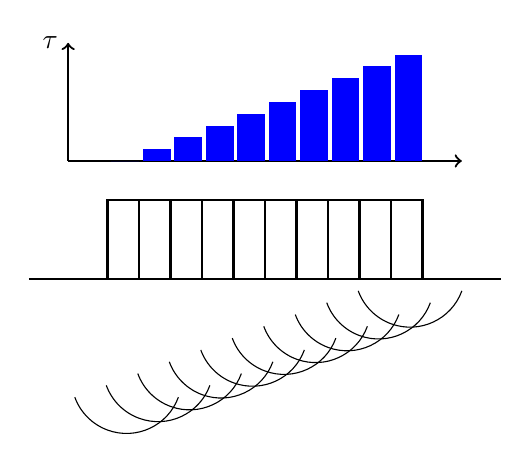
\begin{tikzpicture}
        
        \draw[thick] (-3,0) -- (3,0);
        \draw[thick, ->] (-2.5,1.5) -- (2.5,1.5);
        \draw[thick, ->] (-2.5,1.5) -- (-2.5,3) node[left] {$\tau$};
        
        \foreach \i in {0,...,9} {
            \draw[thick] (-2+.4*\i,0) rectangle ++(.4,1);
            \fill[color=blue] (-2+.4*\i+.05,1.5) rectangle ++(.35,.15*\i);
            \draw (-1.8+.4*\i,-1.5+.15*\i) ++(0:.7) arc (-20:-160:.7);
        }
    \end{tikzpicture}
    \caption{La focalisation, les motifs ou la direction du faisceau dépendent de la loi de retard ($\tau$) appliquée aux éléments du transducteur multi-éléments.}
    \label{me:delay_law}
\end{figurehere}

\section{Échantillon et protocole expérimental}

\subsection{Protocole}

Différentes possibilités existent pour le contrôle de pièce \textit{via} un système multi-éléments. Le choix d'une loi de retard appropriée et les effets de \textit{beam steering} qui s'ensuive permettent la réalisation de différents types de balayages. Dans la suite, un balayage sectoriel a été utilisé (voir figure~\ref{me:fig:sectoriel}).

\begin{figurehere}
    \centering
    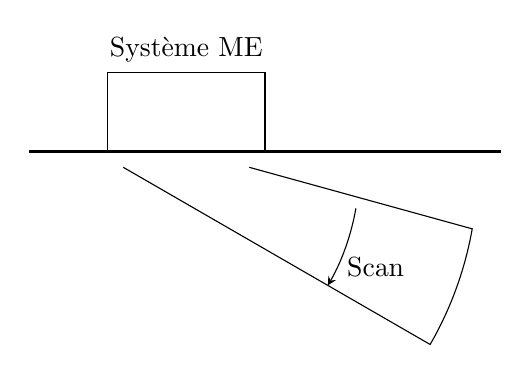
\begin{tikzpicture}[>=stealth]
        % surface
        \draw[thick] (-3,0) -- ++(6,0);
        
        % ME
        \draw (-2,0) rectangle ++(2,1);
        \node (me_capt) at (-1,1.3) {Système ME};
        
        \draw (-1.8,-.2) -- ++(-30:4.5) arc (-30:-10:4.5) -- (-.2,-.2);
        \draw[<-] (-1.8,-.2) ++(-30:3) arc (-30:-10:3) node[near start, right] {Scan};
        
    \end{tikzpicture}
    \caption{Principe du scan sectoriel}
    \label{me:fig:sectoriel}
\end{figurehere}

Une solution efficace est de réaliser l'inspection en plusieurs temps :

\begin{enumerate}
    \item un premier balayage sur toute la longueur de la zone à inspecter, sans affiner l'acquisition permet de positionner grossièrement les défauts.
    \item des balayages plus fins sont effectués ensuite sur les zones présentant potentiellement un défaut.
    \item Au besoin, afin de caractériser au mieux le défaut présent, il est possible de réaliser d'autres balayages, perpendiculairement au premier, ou de modifier les paramètres de \textit{beam steering} pour analyser plus en profondeur ou aller chercher un détail.
\end{enumerate}

\subsection{Plaque}

La plaque utilisée pour les manipulations comprenait une série de défauts positionnés.
La documentation fournie avec la pièce est retranscrite en figure~\ref{me:fig:defauts} et en table~\ref{me:table:defauts}.

\begin{figurehere}
    \centering
    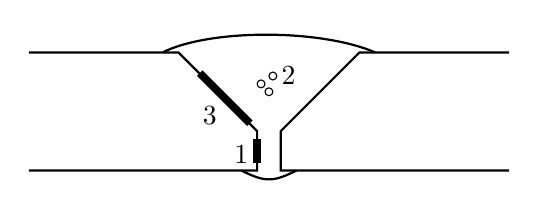
\begin{tikzpicture}
        % plate & cuts
        \draw[thick] (-3,0) -- (-.1,0) -- ++(0,.5) -- ++(-1,1) -- (-3,1.5);
        \begin{scope}[xscale=-1, shift={(-.1,0)}]
            \draw[thick] (-3,0) -- (-.1,0) -- ++(0,.5) -- ++(-1,1) -- (-3,1.5);
        \end{scope}
        
        % weld
        \draw[thick] (-1.3,1.5) .. controls (-.7,1.8) and (.7,1.8) .. (1.4,1.5);
        \draw[thick] (-.3,0) .. controls (0,-.15) and (.1,-.15) .. (.4,0);
        
        %defaults
        \fill[color=black] (-.15,.1) rectangle (-.05,.4);
        \begin{scope}[shift={(-.05,.6)},rotate=45]
            \fill[color=black] (-.15,.1) rectangle (-.05,1);
        \end{scope}
         
        \draw (.05,1) circle (.05);
        \draw (.1,1.2) circle (.05);
        \draw (-.05,1.1) circle (.05);
        
        \node (crack) at (-.3,.2) {1};
        \node (porosity) at (.3,1.2) {2};
        \node (rootfu) at (-.7,.7) {3};
    \end{tikzpicture}
    \caption{Positionnement des défaut au sein du cordon de soudure (vue en coupe projetée)}
    \label{me:fig:defauts}
\end{figurehere}

\begin{tablehere}[H]
	\centering
	\begin{tabular}{c|c|c}
		Numéro & Type & Position (mm) \\\hline
		1 & Fissure & 40\\ 
		2 & Porosité & 117\\
		3 & Manque de fusion & 240 \\
	\end{tabular}	
	\caption{\label{me:table:defauts}Défauts présents et leur position par rapport au bord de la plaque.}
\end{tablehere}

\section{Mesures}

Les mesures sont réalisées au moyen d'un boîtier Sofranel et d'un capteur multi-éléments.

Les résultats sont présentés en figure~\ref{me:measures}.

Sans connaissance \textit{a priori} des défauts il est difficile de les identifier et c'est là que l'expérience de l'expérimentateur est extrêmement importante.
Les différents réglages mis en oeuvre (parcours, zone de focalisation, type de balayage, etc...) peuvent rendre certains défauts parfaitement invisibles et il est important, lors de la préparation d'un contrôle par multi-éléments de considérer ces effets.

\begin{figure*}[!h]
\centering
\begin{subfigure}{0.43\textwidth}
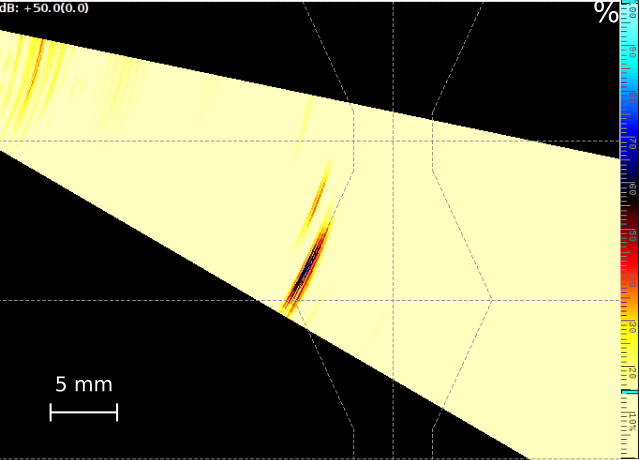
\includegraphics[width=\textwidth]{me_figs/def1.png}
\caption{Fissure --- Copie d'écran}
\end{subfigure}~%
\begin{subfigure}{0.55\textwidth}
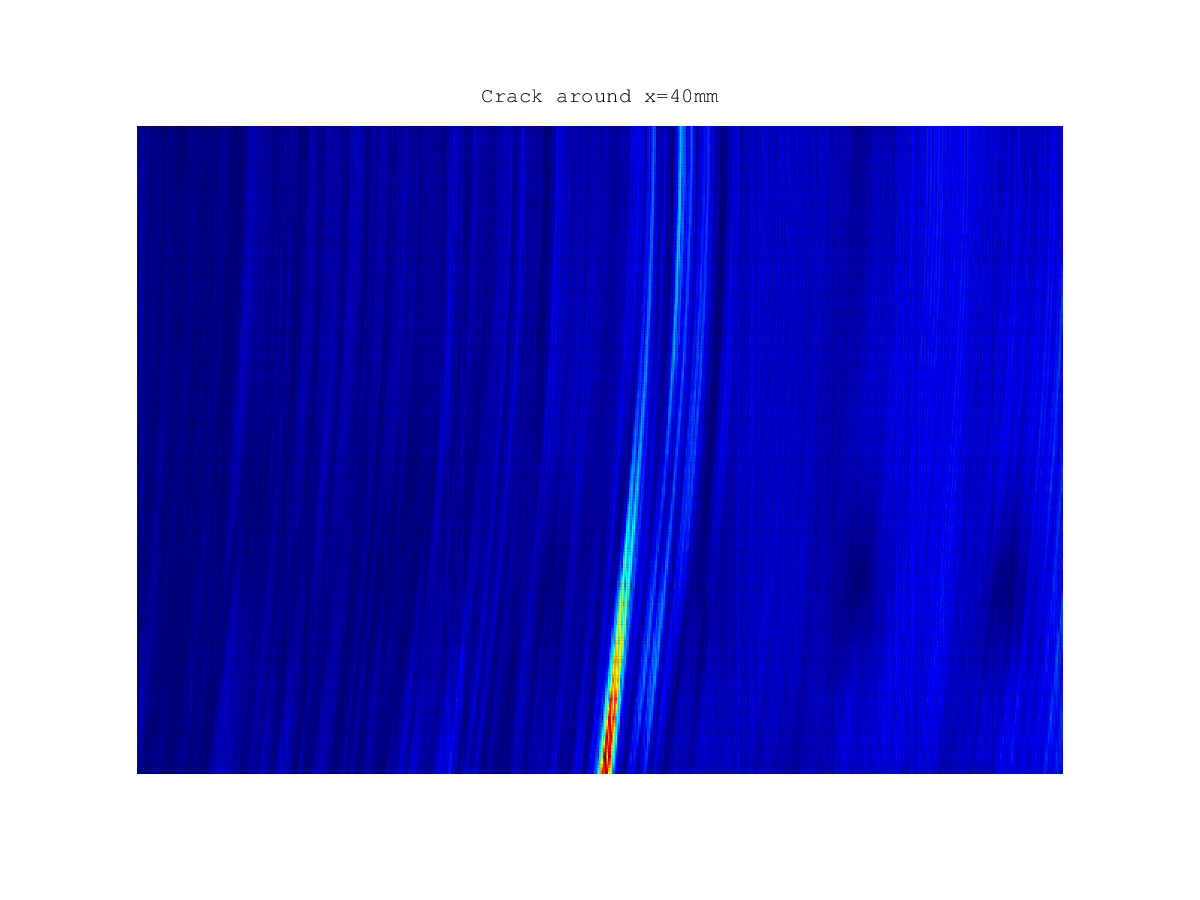
\includegraphics[width=\textwidth]{me_figs/crack_measure.png}
\caption{Fissure --- Données brutes}
\end{subfigure}\\
\begin{subfigure}{0.43\textwidth}
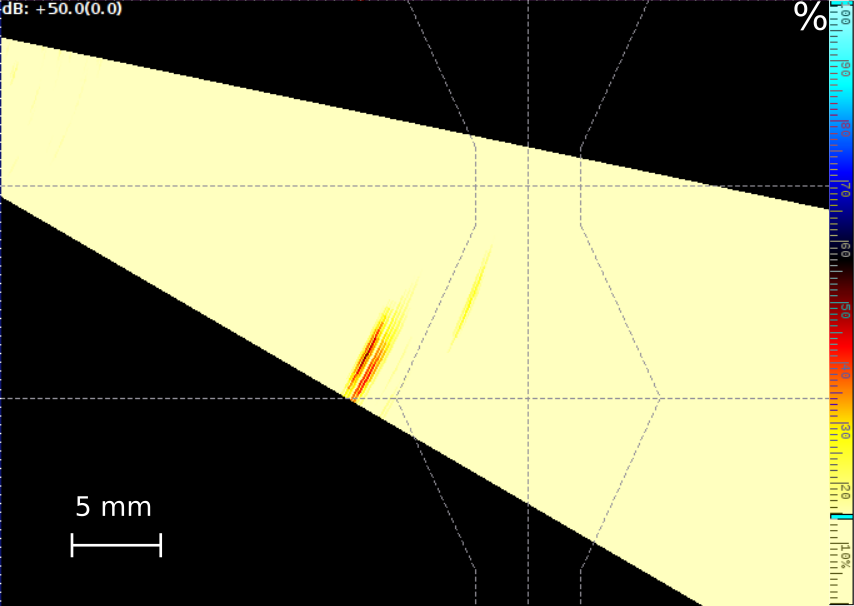
\includegraphics[width=\textwidth]{me_figs/def2.png}
\caption{Porosité --- Copie d'écran}
\end{subfigure}~%
\begin{subfigure}{0.55\textwidth}
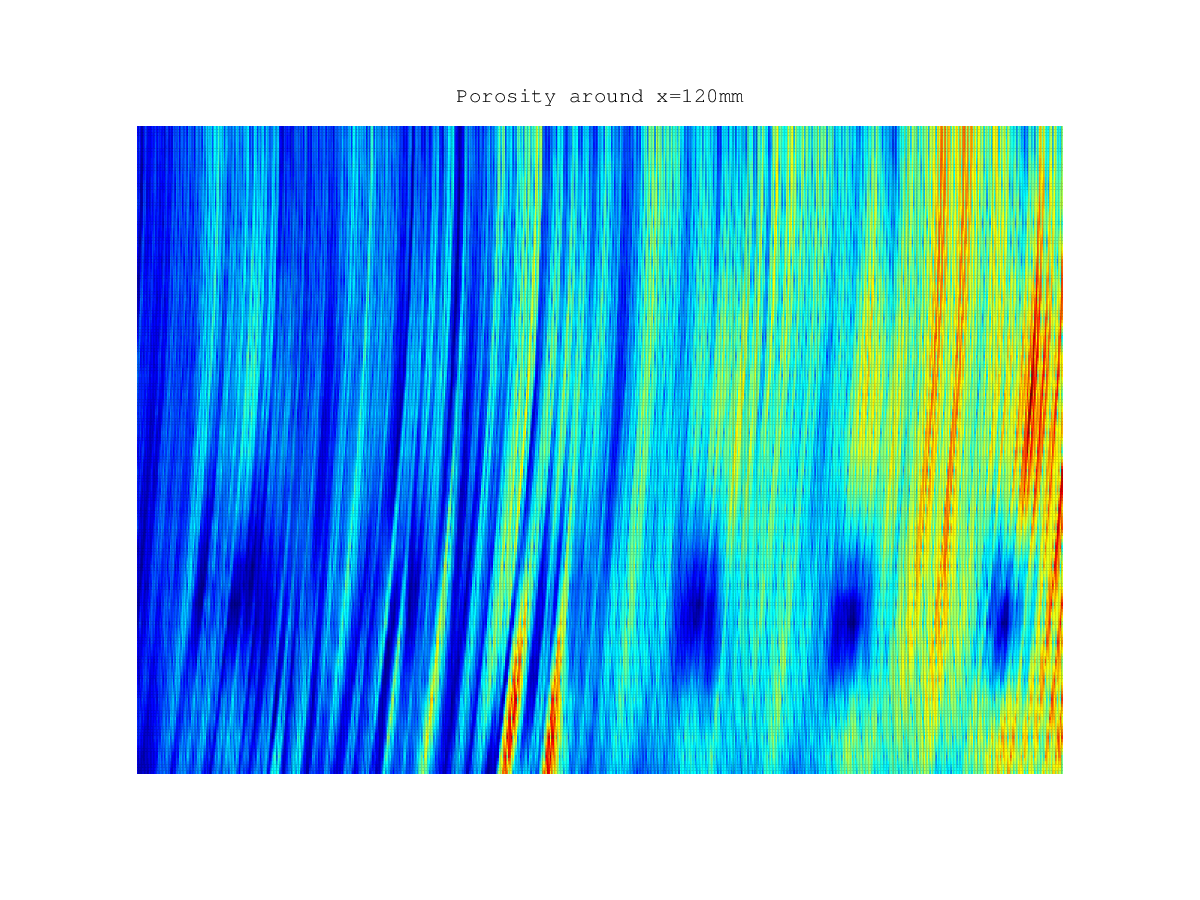
\includegraphics[width=\textwidth]{me_figs/porosity_measure.png}
\caption{Porosité --- Données brutes}
\end{subfigure}\\
\begin{subfigure}{0.43\textwidth}
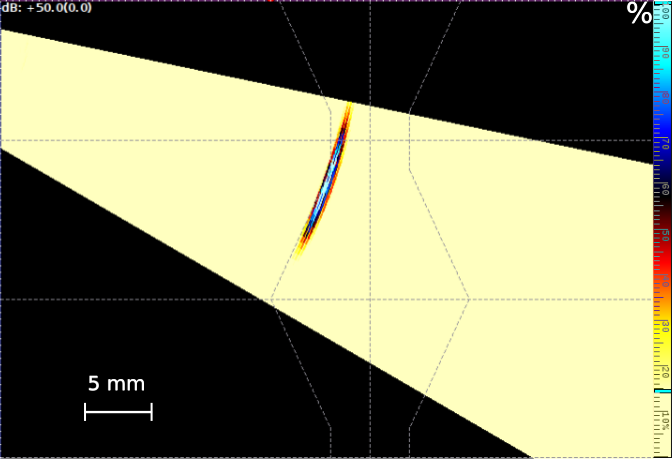
\includegraphics[width=\textwidth]{me_figs/def3.png}
\caption{Manque de fusion --- Copie d'écran}
\end{subfigure}~%
\begin{subfigure}{0.55\textwidth}
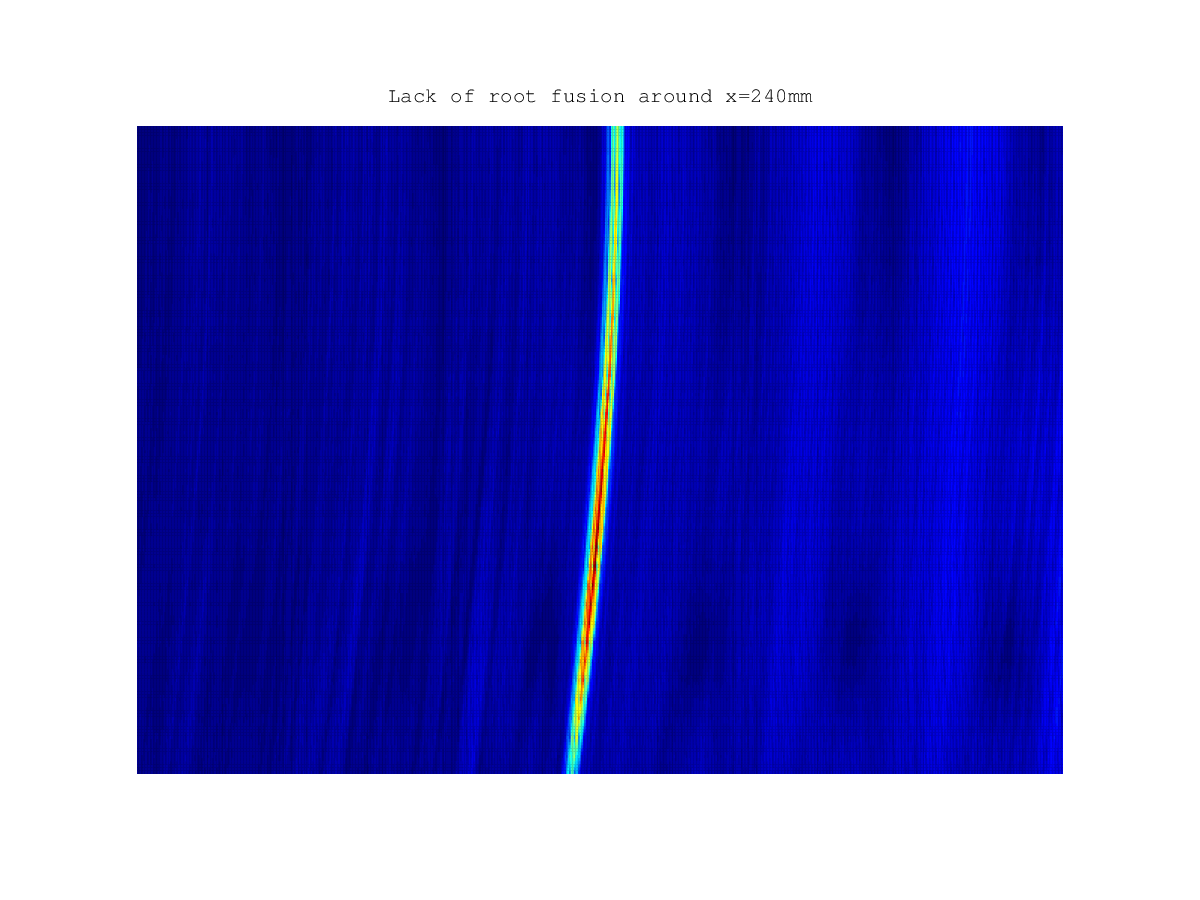
\includegraphics[width=\textwidth]{me_figs/fusion_measure.png}
\caption{Manque de fusion --- Données brutes}
\end{subfigure}\\
\caption{Images obtenues lors de l'inspection. A gauche des copies d'écran du boîtier de contrôle au niveau des défauts (réalisées par A. Dinsenmeyer et T. Lechat) ; à droite, l'affichage des mêmes défaut à partir des données extraites dans GNU/Octave.\label{me:measures}}
\end{figure*}

\subsection{Localisation}

Lors des mesures, les défauts ont été localisés dès le premier scan et les emplacements correspondaient parfaitement à ceux indiqués par la documentation de la pièce d'essai.

Des scans plus localisés ont permis de caractériser aussi bien le type de défaut que son étendue et ce pour chacun des 3 cas.

Les techniques multi-éléments, si elles demandent un réglage et une analyse plus complète, permettent de vraiment représenter les défauts et de les caractériser avec une grande précision.

\section*{Conclusion}

Cette séance a permis de comprendre le fonctionnement des transducteurs multi-éléments et leur intérêt dans le contrôle non-destructif.

Les possibilités de choix du motif de focalisation et de son éventuel déplacement font des méthodes multi-éléments un outil très puissant.

Ces avantages immenses sont malheureusement contre-balancés par le prix élevé des capteurs et des boîtiers d'acquisition et la difficulté de prise en main.

Comme beaucoup de techniques dans le domaine du contrôle, l'expérience et le savoir-faire de l'opérateur joue un rôle non négligeable.